\question Is there an Eulerian Tour? If so, find one. Repeat for an 
Eulerian Path. \newline

\begin{figure}[h]
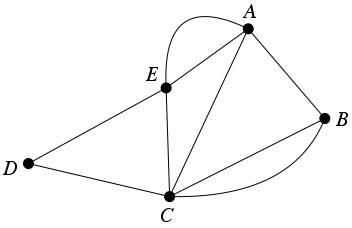
\includegraphics{find_tour}
\centering
\end{figure}

\begin{solution}[0.2in] There is no Eulerian Tour in the graph, because 
not all vertices have an even degree. An Eulerian Tour must visit every 
edge and end up at the same vertex. So the number of times it leaves/enters 
the start vertex must be even (every time it leaves, it must come back). 
Now every other vetex, must have the same condition. Since our tour 
doesn't end at any of these vertices, every time the tour enters a vertex, 
it must leave that vertex. Therefore, every vertex must have an even 
degree for there to be an Eulerian Tour. \newline
There is an Eulerian Path. An Eulerian Path is almost like an Eulerian 
Cycle, without the condition that the start and end vertices must be 
the same. Therefore there are two vertices where the path can leave, 
and not return or enter and not leave. So there can be 2 vertices of 
odd degree. This graph does have 2 vertices of odd degree. 
\[B \rightarrow C \rightarrow D \rightarrow E \rightarrow A 
\rightarrow E \rightarrow C \rightarrow A \rightarrow B \rightarrow C\]
\end{solution}